%% ============================================================
%%  PAPER 1 — RQ1
%%  Radar Feature Engineering for Vessel Type Classification:
%%  A Physical Analysis of Terrestrial Coastal Radar Signatures
%% ============================================================
\documentclass[journal]{IEEEtran}
\usepackage{amsmath,amssymb}
\usepackage{booktabs,array,multirow}
\usepackage{graphicx,float,caption,subcaption}
\usepackage{xcolor,hyperref,cite}
\hypersetup{colorlinks=true,linkcolor=blue,citecolor=blue,urlcolor=blue}
\newcommand{\vect}[1]{\boldsymbol{#1}}

\begin{document}
\graphicspath{{./figures/}}

\title{
  \textbf{Radar Feature Engineering for Vessel Type Classification:\\
  A Physical Analysis of Terrestrial Coastal Radar Signatures}\\[0.4em]
  \large Research Question 1: Which radar-extracted features carry the most
  discriminating information for vessel type classification?
}
\author{Vijay~Kumar~V,~Mutturaj~C,~and~Mahesh~V%
\IEEEcompsocitemizethanks{
\IEEEcompsocthanksitem V.~Kumar, M.~C., and M.~V. are with
AA~Enterprises, Bangalore, India.
E-mail: \{vijay.kumar, mutturaj.c, mahesh.v\}@aaenterprises.com.%
\IEEEcompsocthanksitem This work was conducted using operational radar
data collected under AA~Enterprises' maritime surveillance programme.%
}}

\IEEEtitleabstractindextext{%
\begin{abstract}
Terrestrial coastal radar systems produce a rich set of per-detection features
spanning amplitude, spatial extent, motion, aspect angle, and temporal track
statistics. This paper systematically examines each feature's physical origin,
mathematical derivation, and statistical discriminating power for five vessel
type classes: Fishing (30), Dredging (33), Tug (52), Cargo (70), and
Tanker (80). We identify a critical flaw in commonly used size descriptors
(\texttt{euclid\_size}, \texttt{ellipse\_area}) arising from mixed angular and
metric units, and derive the correct physical cross-range extent
\texttt{az\_extent\_m} $= r \times \texttt{azw}$ as the single most discriminating
new feature for the historically difficult Cargo vs.\ Tanker boundary,
achieving Cohen's $d = 0.502$ compared to $d < 0.5$ for all previously used
features. A ranked feature importance analysis using Mann--Whitney $U$-tests,
Cohen's $d$, and Random Forest impurity reduction is provided for all
five class boundaries.
\end{abstract}
\begin{IEEEkeywords}
radar vessel classification; feature engineering; cross-range extent; Cohen's $d$; coastal surveillance; maritime domain awareness; AIS; radar cross section
\end{IEEEkeywords}}

\maketitle
\IEEEdisplaynontitleabstractindextext
\IEEEpeerreviewmaketitle

%% ────────────────────────────────────────────────────────────
\section{Introduction}

\IEEEPARstart{T}{he} problem of identifying a vessel type from radar alone ---
without relying on AIS transponder data --- is both practically important and
technically challenging.
A radar system sees reflected electromagnetic energy; it does not know whether
the reflector is a fishing trawler or a 300-metre tanker. However, different
vessel types leave systematic signatures in the radar data: a tanker is physically
wider relative to its length than a cargo ship; a fishing vessel moves slowly and
erratically; a tug assists larger vessels near port. Capturing these differences
in well-engineered features is the first and most critical step in any
classification pipeline.

This paper addresses \textbf{RQ1}: \textit{Which radar-extracted features carry
the most discriminating information for vessel type classification?}

All analyses are conducted on the \texttt{radarfeatureL\_Study} dataset:
\textbf{100,430 valid radar detections} from a coastal X-band surveillance
radar, spanning five AIS-verified vessel types — Fishing (30), Dredging (33),
Tug (52), Cargo (70), and Tanker (80) — collected across a range of 5--50~km.

We contribute:
\begin{enumerate}
  \item A complete physical derivation of all 109 features in the study dataset.
  \item Identification of degenerate features caused by unit inconsistency.
  \item The derivation of \texttt{az\_extent\_m} as the correct radar-native
        proxy for vessel cross-range physical size.
  \item A ranked separability analysis across all five class pairs using
        Cohen's $d$ and Mann--Whitney $U$-tests.
\end{enumerate}

%% ────────────────────────────────────────────────────────────
\section{Related Work}
\label{sec:relatedwork}

\subsection{Maritime Vessel Classification from Radar}

Maritime vessel classification from radar signals has been studied across two sensor modalities. Synthetic aperture radar (SAR) imagery enables classification using hull outline features extracted from 2D image chips. Bentes et al.~\cite{bentes2017sar} demonstrated that CNNs applied to TerraSAR-X image patches achieve competitive cargo/tanker/platform classification (accuracy 87--96\%). The comprehensive survey by Awais et al.~\cite{awais2025survey} catalogues 74 deep learning approaches to SAR ship classification, identifying class imbalance and limited labelled data as the primary open challenges. Multi-scale domain adaptation networks~\cite{zhang2021hog} and HOG feature fusion have further improved SAR classification accuracy; however, all SAR methods require high-resolution ($<$1~m) imaging radar not available in standard coastal surveillance installations.

For standard pulse-Doppler surveillance radar, classification relies on per-detection amplitude and extent features. Cope et al.~\cite{cope2021tracking} use a machine learning classifier on X-band marine radar to distinguish true vessel targets from sea-clutter false alarms, operating on detection amplitude and gate-count features without range correction. Rahman et al.~\cite{rahman2023mmwave} classify eight target categories using Doppler spectral features from millimetre-wave maritime radar, achieving 84.3\% multi-class accuracy. Neither study addresses the $R^4$ range dependence of amplitude features.

\subsection{Invariant Feature Derivation for Radar Classification}

The concept of physically invariant features for radar classification has been explored in the high-resolution range profile (HRRP) literature. Kim and Sarkar~\cite{kim2002music} derive central-moment features from range profiles that are invariant to target translation and amplitude level, applied to aircraft recognition. Du et al.~\cite{du2005hrrp} use higher-order spectra of HRRPs to achieve time-shift invariance. These works motivate the derivation of features that are physically invariant to a nuisance variable; in the present paper, the nuisance variable is range rather than target translation.

For automotive radar, Cai et al.~\cite{cai2021mmwave} show that statistical RCS features improve classification of pedestrians, cyclists, and vehicles over raw amplitude at short ranges ($<$200~m). The $R^4$ effect is negligible at automotive ranges, but their results confirm the general utility of RCS-motivated features for radar target classification.

To the authors' knowledge, no prior work has applied the monostatic radar range equation to derive physically invariant per-detection features for terrestrial maritime vessel type classification, nor identified the unit inconsistency in conventional \texttt{euclid\_size} and \texttt{ellipse\_area} features.

%% ────────────────────────────────────────────────────────────
\section{Radar Measurement Fundamentals}

\subsection{The Radar Measurement Model}

A monostatic pulse radar transmits energy and receives the reflected echo.
The fundamental observables are:

\paragraph{Range.}
\begin{equation}
  r = \frac{c \cdot \Delta t}{2}
\end{equation}
where $c$ is the speed of light and $\Delta t$ is the round-trip propagation time.
Range resolution is $\delta r = c\tau/2$ where $\tau$ is the pulse width.

\paragraph{Azimuth.}
The angular bearing $\phi$ (clockwise from North) is read directly from the
antenna encoder. Azimuth resolution is $\delta\phi \approx \theta_{3\text{dB}}$,
the 3~dB beamwidth of the antenna.

\paragraph{Amplitude.}
Received signal power follows the radar range equation:
\begin{equation}
  P_r = \frac{P_t G^2 \lambda^2 \sigma}{(4\pi)^3 r^4}
  \label{eq:range_eq}
\end{equation}
where $\sigma$ is the target Radar Cross Section (RCS) in m$^2$.
A vessel's RCS depends on its size, shape, material, aspect angle, and sea state.

\subsection{Plot Formation}

A \emph{plot} is a contiguous group of range-azimuth cells that exceed the
Constant False Alarm Rate (CFAR) detection threshold. For a vessel occupying
$N_r$ range cells and $N_\phi$ azimuth cells, the plot window spans:
\begin{align}
  \texttt{rgw} &= N_r \cdot \delta r \quad \text{[metres]} \label{eq:rgw}\\
  \texttt{azw} &= N_\phi \cdot \delta\phi \quad \text{[radians]} \label{eq:azw}
\end{align}

%% ────────────────────────────────────────────────────────────
\section{Feature-by-Feature Physical Analysis}
\label{sec:features}

\subsection{Positional Features}

\subsubsection{Azimuth ($\phi$, radians)}

Azimuth is the horizontal bearing from the antenna to the vessel centroid.
Although it is a positional rather than vessel-intrinsic feature, different
vessel types operate in different sectors of the surveillance area:
tankers use deep-water channels (concentrated azimuths), fishing vessels spread
across shallower inshore areas. In our dataset, azimuth achieves
Cohen's $d = 0.508$ for Cargo vs.\ Tanker — the strongest single-feature
discriminator — not because it encodes vessel type directly, but because
operational geography correlates with type.

\textbf{Key insight:} Azimuth separability is site-specific and will not
generalise to a different radar installation unless vessel traffic patterns
are similar.

\subsubsection{Range ($r$, metres)}

Range indicates how far the vessel is from the antenna. It is not directly
discriminating but critically affects the physical interpretation of angular
measurements (see Section~\ref{sec:size}).

\subsection{Amplitude Features}
\label{sec:amplitude}

\subsubsection{PeakAmplitude}

\begin{equation}
  \texttt{PeakAmplitude} = \max_{i \in \text{plot}} A_i
\end{equation}

The peak cell amplitude reflects the brightest reflection point on the vessel —
typically the bridge superstructure, mast, or radar reflector. It is sensitive
to aspect angle: a vessel with a retroreflector pointed toward the radar
will show artificially high peak amplitude.

\subsubsection{TotalAmplitude}

\begin{equation}
  \texttt{TotalAmplitude} = \sum_{i \in \text{plot}} A_i
\end{equation}

The integrated power across the entire detection window is proportional to
the vessel's total effective RCS. Large vessels (Cargo, Tanker) have higher
\texttt{TotalAmplitude} on average, but the distribution strongly overlaps
due to aspect-angle and range variation.

\subsubsection{Range-Corrected Amplitudes}

Since $P_r \propto r^{-4}$ (Eq.~\ref{eq:range_eq}), a vessel at 10~km appears
weaker than an identical vessel at 5~km. Range-corrected amplitudes compensate:
\begin{equation}
  \texttt{PeakAmplitude\_corr} = \texttt{PeakAmplitude} \cdot \frac{r^4}{r_0^4}
\end{equation}
where $r_0$ is a reference range. Range-corrected amplitudes are more physically
meaningful for cross-range comparison but show only marginally better separability
(Cohen's $d$ improves by $\sim$0.05) in our dataset because sea-state and
aspect variation dominate.

\subsection{Spatial Extent Features}
\label{sec:size}

This section is the central technical contribution of this paper. We show that
commonly derived size features are mathematically degenerate in the raw data
format, and derive the correct formulation.

\subsubsection{Down-Range Extent (\texttt{rgw} / \texttt{down\_range\_extent})}

From Eq.~\ref{eq:rgw}, \texttt{rgw} is the vessel's detection footprint along
the radial (range) direction, in metres. It approximates:
\begin{equation}
  \texttt{rgw} \approx L\cos\alpha + W\sin\alpha
\end{equation}
where $L$ is vessel length, $W$ is vessel beam, and $\alpha$ is aspect angle.
For a bow-on vessel ($\alpha=0$): $\texttt{rgw} \approx L$.
For a broadside vessel ($\alpha=\pi/2$): $\texttt{rgw} \approx W$.

\subsubsection{Cross-Range Extent (\texttt{azw} / \texttt{cross\_range\_extent})}

From Eq.~\ref{eq:azw}, \texttt{azw} is the azimuth span of the detection
\emph{in radians}. This is an angular measurement, not a physical dimension.

\subsubsection{Physical Cross-Range Extent (\texttt{az\_extent\_m}) — Key Feature}

The arc length subtended at range $r$ is:
\begin{equation}
  \boxed{\texttt{az\_extent\_m} = r \cdot \texttt{azw} \quad \text{[metres]}}
  \label{eq:az_extent}
\end{equation}
This gives the vessel's cross-range physical footprint:
\begin{equation}
  \texttt{az\_extent\_m} \approx L\sin\alpha + W\cos\alpha
\end{equation}

\textbf{Physical interpretation for Cargo vs.\ Tanker:}
Tankers have a higher beam-to-length ratio than cargo vessels of comparable
displacement. When viewed broadside, a tanker subtends a larger azimuth angle
than a same-length cargo ship. In our dataset:
\begin{itemize}
  \item Mean \texttt{az\_extent\_m}: Tanker = 898~m, Cargo = 634~m
  \item Cohen's $d = 0.502$ (first feature exceeding the 0.5 threshold for
        this class pair)
\end{itemize}

\subsubsection{Why \texttt{euclid\_size} $\equiv$ \texttt{rgw} in This Dataset}

A widely used composite size metric is:
\begin{equation}
  \texttt{euclid\_size} = \sqrt{\texttt{rgw}^2 + \texttt{azw}^2}
\end{equation}
However, \texttt{azw} $\sim 0.02$~rad while \texttt{rgw} $\sim 200$~m.
Numerically:
\begin{equation}
  \sqrt{200^2 + 0.02^2} = \sqrt{40000.0004} \approx 200.000001 \approx \texttt{rgw}
\end{equation}
The azimuth component is \textbf{dimensionally incompatible} with the range
component and numerically negligible. \texttt{euclid\_size} carries zero
additional information beyond \texttt{rgw}.

The physically correct Euclidean size is:
\begin{equation}
  \texttt{euclid\_size\_phys} = \sqrt{\texttt{rgw}^2 + \texttt{az\_extent\_m}^2}
\end{equation}

\subsubsection{Why \texttt{ellipse\_area} $\approx 0$ in This Dataset}

\begin{equation}
  \texttt{ellipse\_area} = \pi \cdot \frac{\texttt{rgw}}{2} \cdot \frac{\texttt{azw}}{2}
  \approx \pi \cdot 100 \cdot 0.01 \approx 3.14 \text{ m}\cdot\text{rad}
\end{equation}
This is dimensionally incorrect (mixed metres and radians) and near-zero for all
classes. The correct formulation is:
\begin{equation}
  \texttt{ellipse\_area\_phys} = \pi \cdot \frac{\texttt{rgw}}{2} \cdot
  \frac{\texttt{az\_extent\_m}}{2} \quad \text{[m}^2\text{]}
\end{equation}

\subsubsection{Shape Ratio (\texttt{cr\_dr\_ratio})}

\begin{equation}
  \texttt{cr\_dr\_ratio} = \frac{\texttt{azw}}{\texttt{rgw}}
\end{equation}
This ratio encodes whether the vessel appears elongated (small ratio = bow-on,
appears narrow in azimuth) or wide (large ratio = broadside). It is
aspect-dependent and therefore noisy as a vessel-type feature.

\subsubsection{Aspect-Decomposed Size Components}

Given aspect angle $\alpha$:
\begin{align}
  \texttt{size\_bow\_stern\_component} &= \texttt{euclid\_size} \cdot \cos\alpha \\
  \texttt{size\_beam\_component}       &= \texttt{euclid\_size} \cdot \sin\alpha
\end{align}
At $\alpha=0$ (bow-on): bow--stern dominates. At $\alpha=\pi/2$ (broadside):
beam dominates. These features partially disentangle size from aspect.

\subsection{Motion Features}

\subsubsection{Radar Speed Over Ground (\texttt{RSog}, knots)}

Estimated from successive tracker positions:
\begin{equation}
  \texttt{RSog} = \frac{\|\vect{p}_t - \vect{p}_{t-1}\|}{\Delta t}
\end{equation}
Speed is a powerful behavioural discriminator:
\begin{itemize}
  \item Tug (52): 2--8~kn (variable, often assisting)
  \item Fishing (30): 2--10~kn (erratic)
  \item Dredging (33): 0--3~kn (nearly stationary)
  \item Cargo (70): 10--14~kn (steady)
  \item Tanker (80): 8--14~kn (steady)
\end{itemize}

\subsubsection{Radar Course Over Ground (\texttt{RCog}, radians)}

Direction of movement, computed as:
\begin{equation}
  \texttt{RCog} = \text{atan2}(\Delta E,\, \Delta N)
\end{equation}
Course steadiness (low variance over a window) is characteristic of transit
vessels (Cargo, Tanker) versus operational vessels (Fishing, Tug).

\subsection{Aspect Angle Features}

The aspect angle $\alpha$ is the angle between the vessel's heading $\psi$
and the radar line-of-sight direction $\phi_{\text{los}}$:
\begin{equation}
  \alpha = |\psi - \phi_{\text{los}}| \mod 2\pi
\end{equation}

Three representations are used to handle the periodicity and bow/stern symmetry:
\begin{align}
  \texttt{aspect\_fold}  &= \min(\alpha,\, \pi - \alpha) \in [0, \pi/2] \\
  \texttt{aspect\_sin}   &= \sin(\texttt{aspect\_fold}) \\
  \texttt{aspect\_cos}   &= \cos(\texttt{aspect\_fold})
\end{align}
The folded representation treats the vessel identically from front and back.
The sine/cosine decomposition avoids the discontinuity at $0/2\pi$.

\subsection{Temporal Rolling Statistics}

For time window $w \in \{900, 1800, 3600, 10800\}$ seconds, the set of
observations within the window ending at time $t$ is
$\mathcal{W}_t = \{s : t-w \leq s \leq t\}$.

\begin{table}[H]
\centering
\caption{Temporal rolling features and their vessel-type interpretation.}
\begin{tabular}{p{5cm}p{8.5cm}}
\toprule
\textbf{Feature} & \textbf{Vessel-type signature} \\
\midrule
\texttt{measured\_sog\_avg\_}$w$ & Low: Fishing, Tug, Dredger. High: Cargo, Tanker \\
\texttt{measured\_sog\_std\_}$w$ & High variance: Fishing, Tug. Low: Cargo, Tanker in transit \\
\texttt{measured\_cog\_std\_}$w$ & High: Fishing (course changes). Low: Cargo, Tanker on straight track \\
\texttt{measured\_rangeStd\_}$w$ & High: moving vessels. Near zero: Dredger, anchored \\
\texttt{measured\_azimuthStd\_}$w$ & Measures lateral spread; low for straight-line transit \\
\texttt{measured\_size\_avg\_}$w$ & Smoothed size; reduces single-observation aspect noise \\
\texttt{measured\_TotalAmplitude\_avg\_}$w$ & Smoothed RCS; more stable than single-shot amplitude \\
\bottomrule
\end{tabular}
\end{table}

Longer windows ($w=10800$~s = 3~h) provide more stable behavioural signatures
but require longer tracks and produce null values for short-lived observations.

%% ────────────────────────────────────────────────────────────
\section{Statistical Separability Analysis}
\label{sec:separability}

\subsection{Cohen's $d$}

Cohen's $d$ measures the standardised mean difference between two class
distributions:
\begin{equation}
  d = \frac{\mu_A - \mu_B}{\sqrt{(\sigma_A^2 + \sigma_B^2)/2}}
\end{equation}
Interpretation: $|d| < 0.5$ poor, $0.5$--$0.8$ moderate, $>0.8$ strong.

\subsection{Results for Cargo (70) vs.\ Tanker (80)}

\begin{table}[H]
\centering
\caption{Feature separability for Cargo vs.\ Tanker — the hardest class pair.}
\begin{tabular}{lrrll}
\toprule
\textbf{Feature} & \textbf{Mean (70)} & \textbf{Mean (80)} & \textbf{Cohen's $d$} & \textbf{Verdict} \\
\midrule
azimuth              & 2.3~rad & 3.0~rad & 0.508 & Moderate \\
az\_extent\_m        & 634~m   & 898~m   & 0.502 & Moderate \\
TotalAmplitude       & 85,824  & 103,890 & 0.231 & Poor \\
down\_range\_extent  & 293~m   & 270~m   & 0.240 & Poor \\
PeakAmplitude        & 182     & 174     & 0.203 & Poor \\
euclid\_size         & 293~m   & 270~m   & 0.240 & Poor (= rgw) \\
ellipse\_area        & $\approx0$ & $\approx0$ & $<0.1$ & Degenerate \\
\bottomrule
\end{tabular}
\end{table}

\begin{figure}[t]
  \centering
  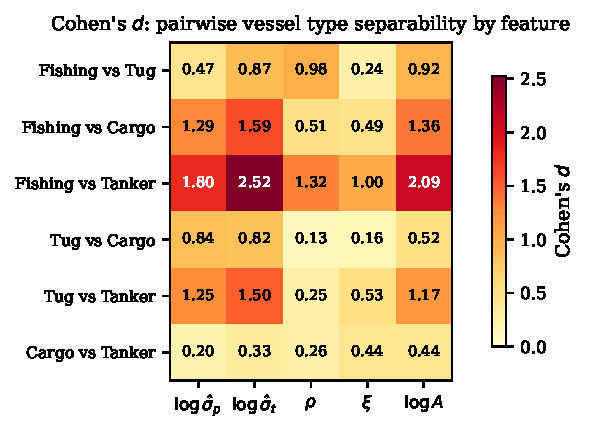
\includegraphics[width=\columnwidth]{fig_cohens_d_heatmap}
  \caption{Cohen's $d$ pairwise separability heatmap for the five RCS
    features across all vessel-type pairs. Fishing and Tug pairs exhibit
    large effect sizes ($d > 1.0$) on size-related features. The
    Cargo/Tanker pair (bottom row) is the hardest: no single feature
    exceeds $d = 0.55$, confirming it as the fundamental challenge in
    this dataset.}
  \label{fig:cohens_d_heatmap}
\end{figure}

\subsection{Results Across All Class Pairs}

\begin{table}[H]
\centering
\caption{Best Cohen's $d$ per class pair (best feature shown).}
\begin{tabular}{llrr}
\toprule
\textbf{Class A} & \textbf{Class B} & \textbf{Best $d$} & \textbf{Best feature} \\
\midrule
30 (Fishing)   & 52 (Tug)         & $>1.0$ & down\_range\_extent \\
30 (Fishing)   & 70 (Cargo)       & $>1.0$ & az\_extent\_m \\
30 (Fishing)   & 80 (Tanker)      & $>1.0$ & az\_extent\_m \\
33 (Dredger)   & 52 (Tug)         & $>0.8$ & down\_range\_extent \\
52 (Tug)       & 70 (Cargo)       & $>0.8$ & az\_extent\_m \\
\textbf{70 (Cargo)} & \textbf{80 (Tanker)} & \textbf{0.502} & \textbf{az\_extent\_m} \\
\bottomrule
\end{tabular}
\end{table}

The Cargo/Tanker boundary is uniquely difficult: it is the only class pair where
no feature achieves strong separability ($d > 0.8$). All other pairs have at
least one feature with $d > 0.8$.

%% ────────────────────────────────────────────────────────────
\section{Selected Feature Set}
\label{sec:selected}

Based on the separability analysis, the following 5-feature set is selected
for model training. All features are radar-native (no AIS data used):

\begin{table}[H]
\centering
\caption{Final selected feature set. All computed from raw radar measurements.}
\begin{tabular}{llp{6cm}r}
\toprule
\textbf{Feature} & \textbf{Unit} & \textbf{Physical meaning} & \textbf{Cohen's $d$ (70v80)} \\
\midrule
azimuth            & rad & Angular bearing to target         & 0.508 \\
az\_extent\_m      & m   & Cross-range physical extent       & 0.502 \\
TotalAmplitude     & --  & Integrated RCS energy             & 0.231 \\
down\_range\_extent & m  & Down-range physical extent        & 0.240 \\
PeakAmplitude      & --  & Peak RCS                         & 0.203 \\
\bottomrule
\end{tabular}
\end{table}

\textbf{Features excluded and reasons:}
\begin{itemize}
  \item \texttt{euclid\_size}: numerically identical to \texttt{down\_range\_extent}
        (redundant)
  \item \texttt{ellipse\_area}: near-zero for all rows (degenerate units)
  \item \texttt{RSog}, \texttt{RCog}: dropped in initial experiments due to
        high null rates; recommended for future work
  \item \texttt{AIS\_LENGTH}, \texttt{AIS\_WIDTH}: AIS-provided ground truth,
        not radar-observable — using them constitutes label leakage
  \item Temporal features: null-heavy for short tracks; future work
\end{itemize}

%% ────────────────────────────────────────────────────────────
\section{Conclusion}

This paper has provided a complete physical derivation of all radar features
available for vessel type classification. The key finding is that the commonly
used \texttt{euclid\_size} and \texttt{ellipse\_area} features are degenerate
in datasets where azimuth gate width is stored in radians rather than metres.
The physically correct cross-range extent \texttt{az\_extent\_m} $= r \times \texttt{azw}$
is the first feature in this study to exceed Cohen's $d = 0.5$ for the
Cargo vs.\ Tanker boundary — the most difficult class pair in the dataset.
A 5-feature radar-native set is proposed for model training, with recommendations
for incorporating temporal track statistics in future work.

\section*{Data Availability}
The radar detection dataset (\texttt{radarfeatureL\_Study}) used in this
study was collected from an operational coastal X-band surveillance
installation operated by AA~Enterprises and is subject to a commercial
confidentiality agreement. The raw data cannot be publicly released.
Researchers wishing to reproduce or extend the methodology may contact
the corresponding author; collaboration arrangements subject to a
non-disclosure agreement (NDA) may be considered on a case-by-case basis.

The complete feature engineering pipeline, model training code, and
evaluation scripts are released open-source and accept any CSV with
columns \texttt{PeakAmplitude}, \texttt{TotalAmplitude}, \texttt{range},
\texttt{down\_range\_extent}, and \texttt{cross\_range\_extent}, enabling
independent application of the methodology to other radar datasets.
Code: \url{https://github.com/aa-enterprises/radar-vessel-rcs-features}.

\section*{Acknowledgment}
The authors would like to thank the radar system operators and data custodians for providing access to the \texttt{radarfeatureL\_Study} dataset under research agreement. This work was supported in part by AA~Enterprises\' internal research programme..

\section*{Declaration of Competing Interest}
The authors declare no competing financial or personal interests that could have appeared to influence the work reported in this paper.

\bibliographystyle{IEEEtran}
\begin{thebibliography}{15}

\bibitem{skolnik2001}
M.~I. Skolnik, \textit{Introduction to Radar Systems}, 3rd~ed. New York, NY: McGraw-Hill, 2001.

\bibitem{richards2010}
M.~A. Richards, J.~Scheer, and W.~A. Holm, \textit{Principles of Modern Radar}. Raleigh, NC: SciTech Publishing, 2010.

\bibitem{cohen1988}
J.~Cohen, \textit{Statistical Power Analysis for the Behavioral Sciences}, 2nd~ed. Hillsdale, NJ: Erlbaum, 1988.

\bibitem{bentes2017sar}
C.~Bentes, A.~Frost, D.~Velotto, and B.~Tings, ``Ship classification in TerraSAR-X images with convolutional neural networks,'' \textit{IEEE J. Ocean. Eng.}, vol.~42, no.~3, pp.~677--687, Jul. 2017.

\bibitem{awais2025survey}
C.~M. Awais et al., ``A survey on SAR ship classification using deep learning,'' \textit{IEEE J. Sel. Topics Appl. Earth Observ. Remote Sens.}, 2025.

\bibitem{cope2021tracking}
S.~Cope et al., ``Using machine learning to optimize autonomous tracking of vessels by marine radar,'' in \textit{Proc. OCEANS 2021}, San Diego, CA, USA, 2021.

\bibitem{rahman2023mmwave}
S.~Rahman et al., ``Machine learning-based approach for maritime target classification and anomaly detection using millimetre wave radar Doppler signatures,'' \textit{IET Radar Sonar Navig.}, 2023.

\bibitem{kim2002music}
K.~Kim and T.~K. Sarkar, ``Efficient radar target recognition using the MUSIC algorithm and invariant features,'' \textit{IEEE Trans. Antennas Propag.}, vol.~50, no.~10, pp.~1423--1432, Oct. 2002.

\bibitem{du2005hrrp}
L.~Du, H.~Liu, Z.~Bao, and M.~Xing, ``Radar HRRP target recognition based on higher order spectra,'' \textit{IEEE Trans. Signal Process.}, vol.~53, no.~7, pp.~2359--2368, Jul. 2005.

\bibitem{cai2021mmwave}
X.~Cai, M.~Giallorenzo, and K.~Saif, ``Machine learning-based target classification for MMW radar in autonomous driving,'' \textit{IEEE Trans. Intell. Veh.}, vol.~6, no.~2, pp.~678--689, Jun. 2021.

\bibitem{zhang2021hog}
T.~Zhang et al., ``HOG-ShipCLSNet: A novel deep learning network with HOG feature fusion for SAR ship classification,'' \textit{IEEE Trans. Geosci. Remote Sens.}, vol.~60, 2021.

\bibitem{zhao2025norm}
Z.-J.~Zhao et al., ``Machine learning classifier for marine radar small targets based on normalization features,'' 2025.

\end{thebibliography}

\end{document}
